\pagebreak
\section{Badania}

\subsection{Funkcja Rastrigina}

\begin{figure}[H]
	\centering
	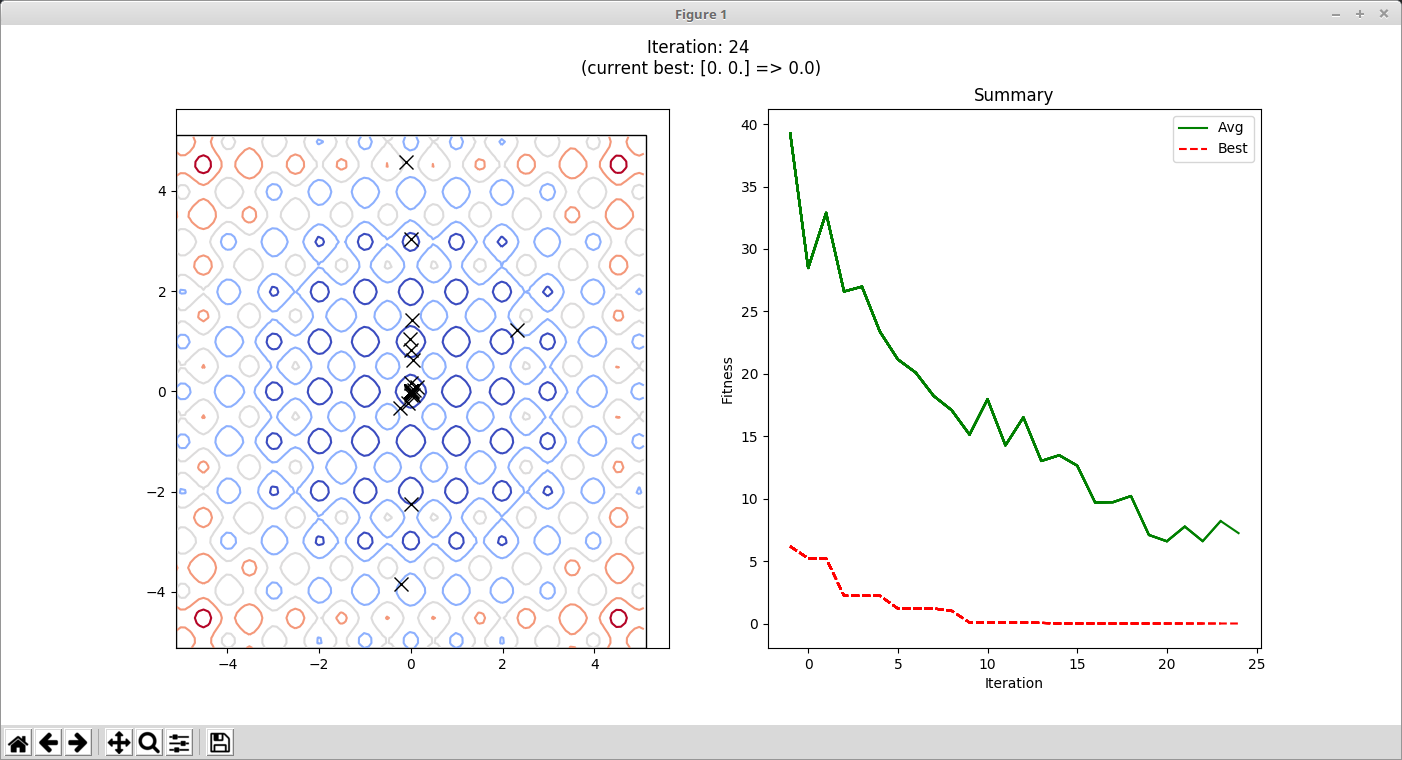
\includegraphics[width=0.7\linewidth]{imgs/program_rastrigin}
	\caption{Testowanie algorytmu PSO, na funkcji Rastrigina.}
	\label{fig:program_rastrigin}
\end{figure}


\subsection{Funkcja Rastrigina z ograniczeniami}

\begin{figure}[H]
	\centering
	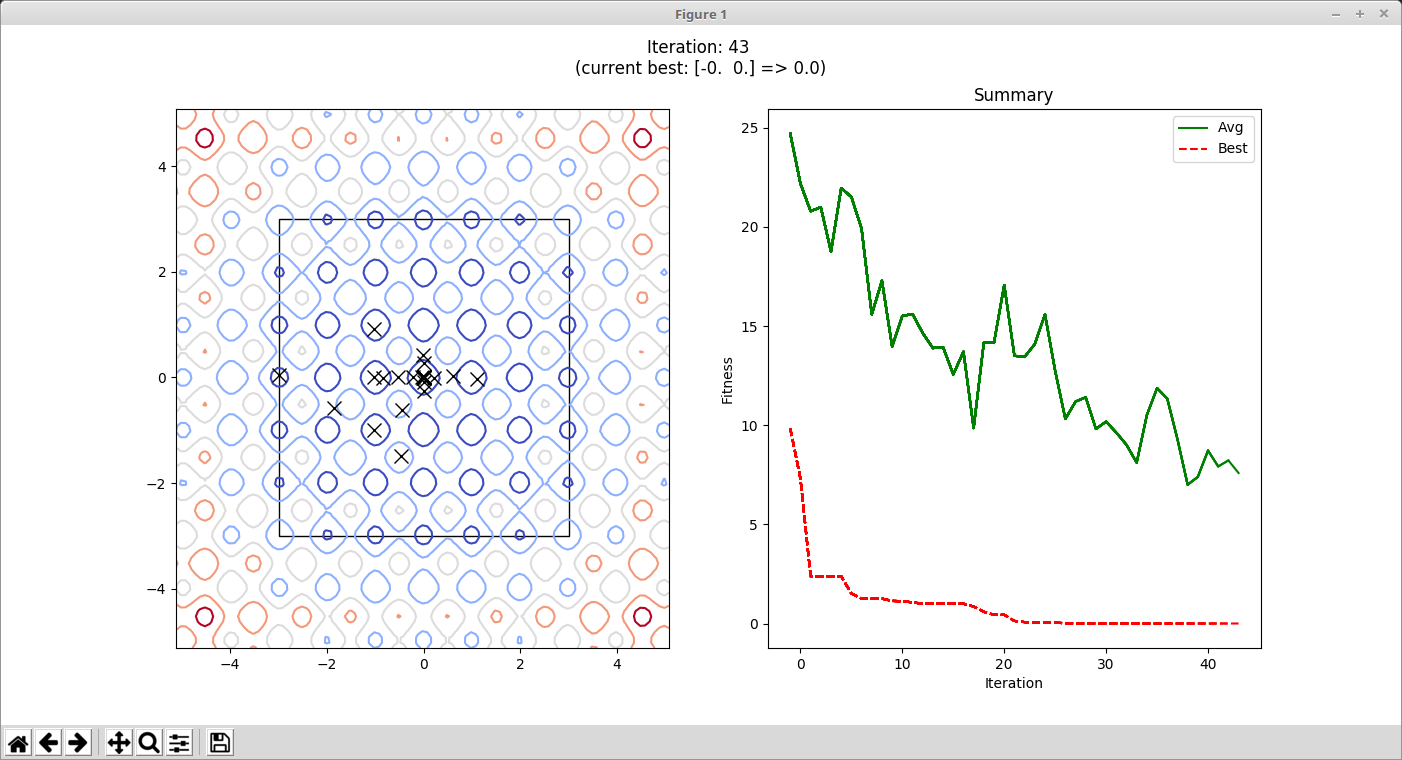
\includegraphics[width=0.7\linewidth]{imgs/program_limited_rastrigin}
	\caption{Testowanie algorytmu PSO, na ograniczonej funkcji Rastrigina.}
	\label{fig:program_limited_rastrigin}
\end{figure}


\subsection{Projektowanie pokoju}

\begin{figure}[H]
	\centering
	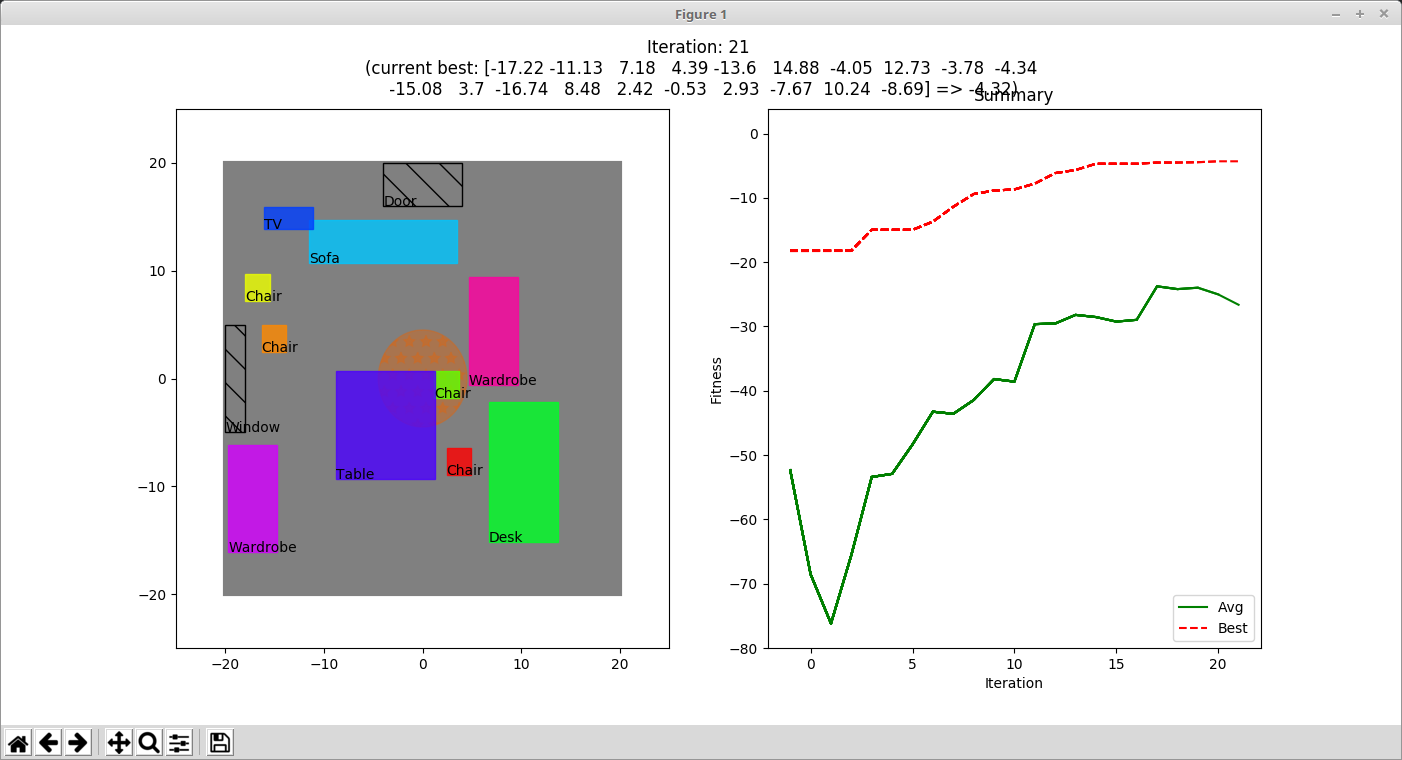
\includegraphics[width=0.7\linewidth]{imgs/program_room}
	\caption{Testowanie algorytmu PSO, przy projektowaniu pokoju.}
	\label{fig:program_room}
\end{figure}


% TODO:
% 4. Wyniki:
% - odpalić każdy z alg. dla każdego problemu z 3-5 razy
% - aggregacje kilku uruchomień